% Source: Lecture21.pdf, pages 1-6. Title on the source: "Van der Waals Theory".
\lecture{21}
\subsection{The van der Waals equation of state}

J.~van der Waals (Nobel Prize, 1910) presented an important approximate equation of state (EOS) for a gas
(1873) that includes two modifications of the ideal gas EOS $pV = N\kB T$. [Equivalently, with $N = nN_A$,
where $N_A = N_{\text{Avogadro}}$, $R = N_A\kB$, so $N\kB = \left(\frac{N}{N_A}\right)(N_A\kB) = nR$, the ideal gas EOS is
$pV = nRT$, where $n = \frac{N}{N_A}$ = \# moles; $\kB = 1.38\times 10^{-23}$~J/Kelvin;
$N_A = 6.02\times 10^{23}$ per mole; $R = 8.314$~J/(mole$\cdot$K).] The van der Waals (vdW) EOS contains two
modifications of the ideal gas EOS:

\paragraph{(1)} A term to incorporate interactions between the molecules or atoms in the gas. For a gas with $N$
particles, there are $\binom N2 = \frac{N(N-1)}{2}$ 2-body interactions, and these are the leading effect. For
$N\gg 1$, $\binom N2\simeq\frac{N^2}{2}$. This term depends on the number density $\rho_n = \left(\frac NV\right)$ and hence
is $\propto\rho_n^2 = \left(\frac NV\right)^2$. At the time that van der Waals proposed his EOS, in 1873, there was no theory
of quantum mechanics; the understanding of this interaction at a fundamental level came later. In the vdW EOS,
$p$ is replaced by $\left[p + a\left(\frac NV\right)^2\right]$, where $a$ is a constant. With $\dim(a)\equiv[a]$:
$\dim(p) = \frac{\text{force}}{\text{area}} = \frac{\text{energy}}{\text{volume}} = \frac EV$, so
$[p] = \frac{[a]}{V^2}\Rightarrow[a] = \frac EV\cdot V^2 = E\cdot V$. Recall that the interaction between the gas
particles (molecules, e.g.\ N$_2$, O$_2$, CO$_2$, \ldots; atoms, e.g.\ Ar, \ldots) is described by the
Lennard-Jones (6--12) potential:
\begin{equation}
  U(r) = U_0\left[\left(\frac{r_0}{r}\right)^{12} - 2\left(\frac{r_0}{r}\right)^6\right],
\end{equation}
where the first term is the short-distance repulsion due to overlap of electron clouds, forcing electrons into
higher-energy states to obey the Pauli exclusion principle, and the second is the long-distance attraction due
to the dipole--dipole interaction. $\mathbf F = -\boldsymbol\nabla U = 0$ at $r = r_0$, the minimum of the
potential energy. An equivalent form is
\begin{equation}
  U(r) = 4U_0\left[\left(\frac\sigma r\right)^{12} - \left(\frac\sigma r\right)^6\right],
\end{equation}
which $=0$ at $r = \sigma$; $r_0 = 2^{1/6}\sigma = 1.12\,\sigma$ (see the plot of $U(r)$ in Lecture~3).
E.g.\ for argon, $r_0 = 3.8\ \text{\AA} = 0.38$~nm and $U_0/\kB = 1.2\times 10^2$~K
($1.16\times 10^4\ \text{K}\leftrightarrow 1\ \text{eV}$); recall the melting temperature $T_m = 83.8$~K, the
boiling temperature $T_b = 87.3$~K, and $T_c = 150.9$~K, $p_c = 4.90\ \text{MPa} = 48.5$~atm.

Since $\dim[a] = E\cdot V$, one expects that
\begin{equation}
  a\sim U_0\cdot(\text{atom or molecule size})^3\sim U_0(\text{few \AA})^3\sim(10^{-2}\ \text{eV})(\text{few \AA})^3 .
\end{equation}

\paragraph{(2)} The other modification of the ideal gas EOS embodied in the vdW EOS is an excluded-volume
correction. The nonzero size of the gas particles is neglected in the ideal EOS, but in reality these particles
do have nonzero size, so the volume available to them is less than $V$;
\begin{equation}
  V_{\text{available}} = V - bN,
\end{equation}
where $\dim(b) = [b]$ = volume; $b\sim(\text{few \AA})^3$. This atomic or molecular size is set by
$a_{\text{Bohr}} = \frac{\hbar}{\alpha m_ec}\simeq 0.53$~\AA, where $\alpha = \frac{e^2}{4\pi\hbar c} = \frac{1}{137}$.

(At the time, 1873, when van der Waals proposed his EOS, neither (1) nor (2) was understood at a fundamental
level; the effect of particle--particle interactions and excluded volume were included in an empirical manner.)
So $pV = N\kB T$ is replaced by the vdW equation of state for a non-ideal gas:
\begin{equation}
  \boxed{\left[p + a\left(\frac NV\right)^2\right]\left[V - bN\right] = N\kB T}.
\end{equation}
We can reexpress this in several ways. It is useful to define (lower-case)
\begin{equation}
  v = \frac VN = \text{volume per particle}
\end{equation}
(N.B.: the number density is $\rho_n = \frac NV = \frac1v$; upper-case $V$, lower-case $v$). Then
\begin{equation}
  \left(p + \frac{a}{v^2}\right)(v-b) = \kB T\ \Rightarrow\ p + \frac{a}{v^2} = \frac{\kB T}{v-b}
  \ \Rightarrow\ \boxed{p = \frac{\kB T}{v-b} - \frac{a}{v^2}}.
\end{equation}

\subsection{The critical point}

Plot curves of constant temperature $T$. At $T\gg T_c$, at low $\rho_n = N/V$, the curve is a hyperbola,
$pV = N\kB T$, i.e.\ $pv = \kB T$. As $T$ decreases to $T_c$, the curve develops a point at $p = p_c$, $v = v_c$
with zero slope; this is also a point of inflection.

\begin{diagram}
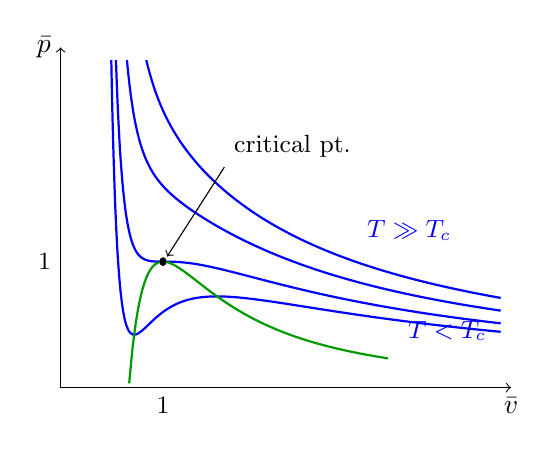
\begin{tikzpicture}[xscale=1.3,yscale=1.6]
  \draw[->] (0,0) -- (4.4,0) node[below] {$\bar v$};
  \draw[->] (0,0) -- (0,2.7) node[left] {$\bar p$};
  \begin{scope}
  \clip (0,0) rectangle (4.3,2.6);
  \foreach \t in {1.3,1.15,1.0,0.9} {
    \draw[thick,blue,domain=0.45:4.3,samples=150,smooth] plot (\x,{8*\t/(3*\x-1) - 3/(\x*\x)});
  }
  \draw[thick,green!60!black,domain=0.67:3.2,samples=80,smooth] plot (\x,{(3*\x-2)/(\x^3)});
  \end{scope}
  \fill (1,1) circle (0.035);
  \draw[->] (1.6,1.75) node[anchor=south west,font=\small] {critical pt.} -- (1.04,1.04);
  \node[blue,font=\small,anchor=west] at (2.9,1.25) {$T\gg T_c$};
  \node[blue,font=\small,anchor=west] at (3.3,0.45) {$T<T_c$};
  \node[left,font=\small] at (0,1) {$1$}; \node[below,font=\small] at (1,0) {$1$};
\end{tikzpicture}
\diagramcaption{Isotherms (constant $T$) of the van der Waals EOS, in reduced units, for temperatures above, at
and below $T_c$. The green curve bounds the region where $\partial p/\partial v>0$. (See also the graph posted
on BrightSpace.)}
\end{diagram}

At the critical point, $\pder pv = 0$ and $\frac{\partial^2p}{\partial v^2} = 0$ (inflection point):
\begin{align}
  0 = \pder pv &= \frac{-\kB T}{(v-b)^2} + \frac{2a}{v^3}\ \Rightarrow\ \frac{\kB T}{(v-b)^2} = \frac{2a}{v^3},\\
  0 = \frac{\partial^2p}{\partial v^2} &= \frac{2\kB T}{(v-b)^3} - \frac{6a}{v^4}\ \Rightarrow\ \frac{\kB T}{(v-b)^3} = \frac{3a}{v^4}.
\end{align}
To solve these equations, substitute the first in the second:
\begin{equation}
  \frac{\kB T}{(v-b)^3} = \frac3v\cdot\frac{a}{v^3} = \frac{3}{2v}\cdot\frac{2a}{v^3} = \frac{3}{2v}\cdot\frac{\kB T}{(v-b)^2}
  \ \Rightarrow\ \frac{1}{v-b} = \frac{3}{2v}\ \Rightarrow\ v-b = \frac23v\ \Rightarrow\ \frac v3 - b = 0
\end{equation}
\begin{equation}
  \Rightarrow\quad\boxed{v = v_c = 3b}.
\end{equation}
Substitute this in the $\partial p/\partial v = 0$ equation:
$\kB T_c = \frac{2a}{v_c^3}(v_c-b)^2 = \frac{2a}{(3b)^3}(2b)^2 = \frac{8a}{27b}$:
\begin{equation}
  \boxed{\kB T_c = \frac{8a}{27b}}.
\end{equation}
Substitute in the EOS:
\begin{equation}
  p_c = \frac{\kB T_c}{v_c-b} - \frac{a}{v_c^2} = \frac{\left(\frac{8a}{27b}\right)}{(2b)} - \frac{a}{(3b)^2}
  = \left(\frac{4}{27}-\frac19\right)\frac{a}{b^2} = \boxed{\frac{a}{27b^2} = p_c}.
\end{equation}
Summary of the critical values of $p$, $T$, $v = \rho_n^{-1}$:
\begin{equation}
  p_c = \frac{a}{27b^2},\qquad \kB T_c = \frac{8a}{27b},\qquad v_c = 3b,\ \text{i.e.}\ (\rho_n)_c = \frac{1}{v_c} = \frac{1}{3b}.
\end{equation}

A standard measure of the comparison with the ideal gas EOS is the ratio
\begin{equation}
  Z_c\equiv\frac{p_cv_c}{\kB T_c};
\end{equation}
this is $=1$ at all points for an ideal gas, including the critical point. For the vdW EOS,
\begin{equation}
  Z_c = \frac{\left(\frac{a}{27b^2}\right)(3b)}{\left(\frac{8a}{27b}\right)} = \frac38 = 0.375 .
\end{equation}
The fact that $Z_c<1$ reflects the effect of the attractive interaction which is responsible for the critical
behavior and condensation of the gas. (The ideal gas EOS does not yield any critical point or condensation.)

From the critical values $p_c$ and $T_c$, we can determine $a$ and $b$:
\begin{gather}
  v_c = 3b = \frac38\frac{\kB T_c}{p_c}\ \Rightarrow\ \boxed{b = \frac{\kB T_c}{8p_c}};\nonumber\\
  a = \frac{27}{8}b\cdot(\kB T_c) = \frac{27}{8}\left(\frac{\kB T_c}{8p_c}\right)(\kB T_c)
  \ \Rightarrow\ \boxed{a = \frac{27}{64}\frac{(\kB T_c)^2}{p_c}}.
\end{gather}
These relations are also often expressed in terms of molar quantities. Recall that \# moles $= n = N/N_A$. The
molar volume is $V_m = \frac Vn = \frac{N_AV}{N}$, so $\frac NV = \frac{N_A}{V_m}$, and
$\left[p + a\left(\frac NV\right)^2\right][V - bN] = N\kB T$ can be rewritten as
$\left[p + a\left(\frac{N_A}{V_m}\right)^2\right][nV_m - bN_An] = nRT$, i.e.\ $\left[p + a\left(\frac{N_A}{V_m}\right)^2\right][V_m - bN_A] = RT$, or
\begin{equation}
  \left[p + \frac{a'}{V_m^2}\right]\left[V_m - b'\right] = RT,\qquad\text{where}\quad a' = N_A^2a\ \text{and}\ b' = N_Ab .
\end{equation}
Then $a' = \frac{27}{64}\frac{(RT_c)^2}{p_c}$ and $b' = \frac{RT_c}{8p_c}$. The ratio $Z_c$ can also be expressed
in terms of molar quantities:
\begin{equation}
  Z_c = \frac{p_cv_c}{\kB T_c} = \frac{p_cN_Av_c}{N_A\kB T_c} = \frac{p_cV_{m,c}}{RT_c},
\end{equation}
where $V_{m,c}$ is the critical value of $V_m$.

\subsection{Law of corresponding states}

It is convenient to express the vdW EOS in terms of the critical quantities. Define
$\bar p = \frac{p}{p_c}$, $\bar T = \frac{T}{T_c}$, $\bar V = \frac{V}{V_c}$, $\bar v = \frac{v}{v_c}$, so
\begin{equation}
  \left(p + \frac{a}{v^2}\right)(v-b) = \kB T\ \Rightarrow\
  \left[\bar pp_c + \frac{a}{(\bar vv_c)^2}\right]\left[\bar vv_c - b\right] = \kB T_c\cdot\bar T;
\end{equation}
substitute the values of $p_c$, $v_c$, and $T_c$:
\begin{gather}
  \left[\left(\frac{a}{27b^2}\right)\bar p + \frac{a}{(3b)^2\bar v^2}\right]\left[(3b)\bar v - b\right] = \left(\frac{8a}{27b}\right)\bar T\nonumber\\
  \Rightarrow\ \left(\frac{a}{27b^2}\right)\left[\bar p + \frac{3}{\bar v^2}\right](3b)\left[\bar v - \frac13\right] = \left(\frac{8a}{27b}\right)\bar T
\end{gather}
\begin{equation}
  \Rightarrow\quad\boxed{\left(\bar p + \frac{3}{\bar v^2}\right)\left(\bar v - \frac13\right) = \frac83\bar T}.
\end{equation}
Note that at the critical point, with $\bar p = \bar p_c = 1$, $\bar v = \bar v_c = 1$, $\bar T = \bar T_c = 1$,
this is an identity: $4\cdot(2/3) = 8/3$.

The vdW EOS in terms of $\bar p$, $\bar v$, and $\bar T$ is called the ``Law of Corresponding States'' and fits
data from many different gases rather well. See, e.g., Fig.~5.3, p.~73 in Stanley's book.

\subsection{Critical exponents of the van der Waals theory}

The vdW EOS yields predictions for critical exponents. To determine these, define the fractional differences in
the reduced $\bar p$, $\bar T$, $\bar v$ from their critical values $\bar p_c = 1$, $\bar T_c = 1$ and
$\bar v_c = 1$:
\begin{equation}
  \delta\bar p = \bar p-1 = \frac{p-p_c}{p_c},\qquad
  \delta\bar T = \bar T-1 = \frac{T-T_c}{T_c} = \tau,\qquad
  \delta\bar v = \bar v-1 = \frac{v}{v_c}-1 .
\end{equation}
Then the vdW EOS, written in terms of these fractional deviations from critical values, is
\begin{equation}\label{eq:vdwdev}
  \left[1+\delta\bar p+\frac{3}{(1+\delta\bar v)^2}\right]\left[1+\delta\bar v-\frac13\right] = \frac83(1+\delta\bar T).
\end{equation}

\paragraph{Critical isotherm.} Recall that the critical isotherm in a liquid--gas system is (with
$\rho\propto\rho_n = \frac1v$)
\begin{equation}
  \Delta\rho = \rho_\ell-\rho_g\propto|p-p_c|^{1/\delta}\quad\text{at } T_c,
\end{equation}
analogous to $M\propto|H|^{1/\delta}$ at $T = T_c$ in a magnetic system. Use
$(1+x)^{-2} = 1-2x+3x^2-4x^3+\Order(x^4)$ and set $\delta\bar T = 0$; then eq.~\eqref{eq:vdwdev} becomes
\begin{align}
  &\left[1+\delta\bar p+3\left\{1-2(\delta\bar v)+3(\delta\bar v)^2-4(\delta\bar v)^3+\Order((\delta\bar v)^4)\right\}\right]
   \left[\frac23+\delta\bar v\right] = \frac83,\nonumber\\
  &\left[4+\delta\bar p-6(\delta\bar v)+9(\delta\bar v)^2-12(\delta\bar v)^3+\Order((\delta\bar v)^4)\right]\cdot\frac23\left[1+\frac32(\delta\bar v)\right] = \frac83,\nonumber\\
  &\frac83\left[1+\frac14\delta\bar p-\frac32(\delta\bar v)+\frac94(\delta\bar v)^2-3(\delta\bar v)^3+\Order((\delta\bar v)^4)\right]\left[1+\frac32(\delta\bar v)\right] = \frac83
\end{align}
\begin{equation}
  \Rightarrow\ \frac14\delta\bar p + \underbrace{\left(-\frac32+\frac32\right)}_{0}(\delta\bar v)
  + \underbrace{\left(\frac94-\frac94\right)}_{0}(\delta\bar v)^2
  + \underbrace{\left(-3+\frac{27}{8}\right)}_{\frac38}(\delta\bar v)^3 + \Order((\delta\bar v)^4) = 0
\end{equation}
\begin{equation}
  \Rightarrow\ \frac14\delta\bar p + \frac38(\delta\bar v)^3 = 0,\qquad \delta\bar p = -\frac32(\delta\bar v)^3;
\end{equation}
since $\delta\bar v\propto-\delta\bar\rho_n\propto-\delta\bar\rho$, $\Rightarrow\delta\bar p = \frac32(\delta\bar\rho)^3$,
$\delta\bar\rho\propto(\delta\bar p)^{1/3}\Rightarrow$ the critical exponent
\begin{equation}
  \boxed{\delta = 3}.
\end{equation}

\paragraph{Compressibility.} Recall that the isothermal compressibility is
$\kappa_T = -\frac1V\left(\frac{\partial V}{\partial p}\right)_T$ and this has the critical behavior
$\kappa_T\sim\tau^{-\gamma}$, $|\tau|^{-\gamma'}$ as $\tau\to 0$, with $\gamma = \gamma'$. Now
$(-V\kappa_T)^{-1} = \left(\frac{\partial p}{\partial V}\right)_T\propto\left(\frac{\partial\bar p}{\partial\bar v}\right)_T$;
calculating this from eq.~\eqref{eq:vdwdev} above, and setting $\delta\bar v = 0$ to get to the critical point, one
finds $\kappa_T^{-1}\propto\delta\bar T = \tau$, so
\begin{equation}
  \boxed{\gamma = \gamma' = 1}.
\end{equation}
In a similar manner, one obtains the value $\boxed{\beta = \frac12}$ for the critical exponent for the order
parameter, $\Delta\rho = \rho_\ell-\rho_g$.

From these critical exponents, all of the others can be calculated, and one finds that vdW yields the same
critical exponents as the Landau--Ginzburg formalism and as mean field theory. Like these approaches to critical
behavior, the vdW EOS is only approximate. Thus, in particular, the critical exponents from vdW do not agree with
the experimentally measured critical exponents for the liquid--gas critical point, which are those of the 3D Ising
universality class (as we motivated earlier from the lattice-gas model of this transition).

\subsection{Unphysical region and the Maxwell construction}

The vdW EOS has an additional deficiency, which is evident from the graphs for the solution of this equation.
Multiplied out, it is a cubic equation in $\bar v$ or $V$ as a function of $p$ for a given $T$. The (isothermal)
compressibility
\begin{equation}
  \kappa_T = -\frac1V\left(\frac{\partial V}{\partial p}\right)_T = -\frac1v\left(\frac{\partial v}{\partial p}\right)_T
\end{equation}
must be a positive quantity since exerting pressure on the system reduces the volume, so
$\frac{\partial v}{\partial p}<0$. Now $\frac{\partial v}{\partial p}<0\Leftrightarrow\frac{\partial p}{\partial v}<0$.
Now $\frac{\partial p}{\partial v}$ is the slope of the curve of $p$ vs.\ $V$. The condition
$\frac{\partial p}{\partial v}<0$ is \emph{not} satisfied for all $v$; it is violated in the region of $v$ and $p$
within the green boundary. So these values of $p$ and $V$ are not physically allowed, contrary to the prediction of
the vdW EOS. (At the critical point, $\partial p/\partial v = 0\Rightarrow\kappa_T = \infty$; this is
understandable since the gas is at the verge of changing to a liquid, analogous to the magnetic susceptibility
$\chi\to\infty$ at $T_c$ in a magnetic system.)

\begin{diagram}
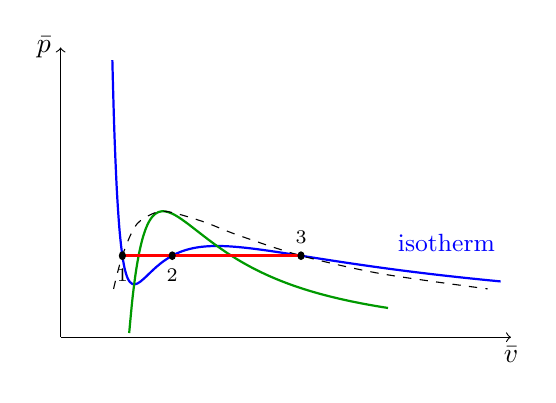
\begin{tikzpicture}[xscale=1.3,yscale=1.6]
  \draw[->] (0,0) -- (4.4,0) node[below] {$\bar v$};
  \draw[->] (0,0) -- (0,2.3) node[left] {$\bar p$};
  \begin{scope}
  \clip (0,-0.3) rectangle (4.3,2.2);
  \draw[thick,blue,domain=0.47:4.3,samples=150,smooth] plot (\x,{8*0.9/(3*\x-1) - 3/(\x*\x)});
  \draw[thick,green!60!black,domain=0.67:3.2,samples=80,smooth] plot (\x,{(3*\x-2)/(\x^3)});
  \draw[dashed] plot[smooth] coordinates {(0.5174,0.3834) (0.5534,0.5045) (0.6034,0.647) (0.6841,0.8119) (0.7755,0.9219) (1,1) (1.3761,0.9219) (1.7271,0.8119) (2.3488,0.647) (3.1276,0.5045) (4.1725,0.3834)};
  \end{scope}
  \draw[very thick,red] (0.6034,0.647) -- (2.3488,0.647);
  \fill (0.6034,0.647) circle (0.035); \fill (1.0905,0.647) circle (0.035); \fill (2.3488,0.647) circle (0.035);
  \node[below,font=\scriptsize] at (0.6034,0.62) {1}; \node[below,font=\scriptsize] at (1.0905,0.62) {2}; \node[above,font=\scriptsize] at (2.3488,0.67) {3};
  \node[blue,font=\small,anchor=west] at (3.2,0.75) {isotherm};
\end{tikzpicture}\qquad
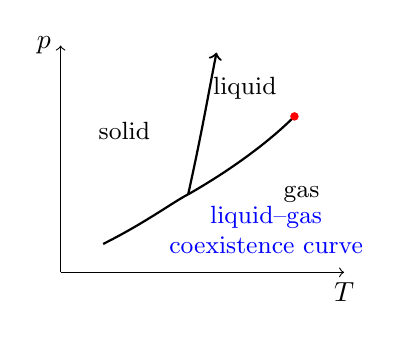
\begin{tikzpicture}[scale=0.9]
  \draw[->] (0,0) -- (4,0) node[below] {$T$}; \draw[->] (0,0) -- (0,3.2) node[left] {$p$};
  \draw[thick] (0.6,0.4) .. controls (1.2,0.7) and (1.6,1.0) .. (1.8,1.1);
  \draw[thick] (1.8,1.1) .. controls (2.5,1.5) and (3,1.9) .. (3.3,2.2);
  \draw[thick,->] (1.8,1.1) .. controls (2,2) and (2.1,2.6) .. (2.2,3.1);
  \fill[red] (3.3,2.2) circle (0.06);
  \node[font=\small] at (0.9,2.0) {solid}; \node[font=\small] at (2.6,2.6) {liquid}; \node[font=\small] at (3.4,1.1) {gas};
  \node[blue,font=\small,align=center] at (2.9,0.6) {liquid--gas\\ coexistence curve};
\end{tikzpicture}
\diagramcaption{Left: the isotherm $\bar T = 0.9$ in reduced units. The three dots show 3 solutions of the cubic vdW
EOS, and the red segment is the liquid--gas coexistence (Maxwell) line; the dashed curve is the coexistence curve in the
$(v,p)$ diagram and the green curve bounds the unphysical region. Right: the corresponding $p$--$T$ phase diagram.}
\end{diagram}

The three dots show 3 solutions of the cubic vdW EOS; the one inside the green region is thermodynamically
unstable, because $\kappa_T<0$. The other two represent different values of $v = V/N$ and hence the number density
$\rho_n = 1/v$ and the (mass) density $\rho\propto\rho_n$; the one at smaller $v$, i.e.\ larger $\rho$, is the
liquid phase and the one at larger $v$, i.e.\ smaller $\rho$, is the gas phase. These coexist along the liquid--gas
coexistence curve (the dashed curve in the $(v,p)$ diagram). This curve is determined by the requirement of
minimizing the Gibbs free energy $G(T,p)$. We have $\dd G = -S\dd T + V\dd p$, so since $\dd T = 0$ on an
isotherm, $\dd G = V\dd p$ on this isotherm. Denote the points 1, 2, 3 as shown. Now the liquid and gas points
across from each other on a phase coexistence curve must have the same (minimized) value of $G$, so
$\int_1^3\dd G = 0$. But
\begin{equation}
  \int_1^3\dd G = \int_1^2\dd G + \int_2^3\dd G = \int_1^2V\dd p + \int_2^3V\dd p,
\end{equation}
so the areas under the curves are equal. This is the ``Maxwell Equal-Area'' construction. So the actual $p$--$V$
curve for stable thermodynamic states is flat between $v_{\text{liq.}}$ and $v_{\text{gas}}$.

\begin{diagram}
\begin{tikzpicture}[scale=0.8]
  \draw (0,0) -- (4.5,0) node[below] {$v$}; \draw (0,0) -- (0,2.8) node[left] {$p$};
  \draw[thick,blue] (0.3,2.6) .. controls (0.5,1.4) and (0.7,1.1) .. (1.1,1.05) -- (2.6,1.05) .. controls (3,0.9) and (3.6,0.6) .. (4.3,0.45);
  \draw (1.1,0.05) -- (1.1,-0.05); \draw (2.6,0.05) -- (2.6,-0.05);
  \node[below,blue,font=\small] at (1.1,0) {$v_{\text{liq.}}$}; \node[below,blue,font=\small] at (2.6,0) {$v_{\text{gas}}$};
\end{tikzpicture}
\diagramcaption{The $p$--$v$ isotherm for stable thermodynamic states, after the Maxwell construction.}
\end{diagram}

Interestingly, there are states between the dashed curve obtained from the Maxwell construction and the green curve
delimiting the unphysical region. These are metastable states. The states on the lower-$v$ (higher-$\rho$) side are
superheated liquid, and the states on the larger-$v$ (i.e.\ smaller $\rho$) side are supercooled gas. These states can
be produced; for example, one can produce superheated water by heating it slightly above $T_b = 100^\circ$C (at
$p = 1$~atm). If the container has no scratches, then the water can stay liquid. Scratches can provide places where
the equilibrium gas phase (bubbles of water vapor) form, and this is why, when the water in a pan first begins to
boil, the bubbles arise from the scratches on the bottom of the pan. Later, once vigorous boiling has begun, the
bubbles appear throughout the full volume of the water.

Supercooling of water vapor also occurs in the atmosphere. Nucleation of H$_2$O molecules produces raindrops.

The same metastability occurs at the liquid--solid phase coexistence curve, which is also a 1st-order boundary. If one
cools water slightly below $T_m = 0^\circ$C, it can remain as a metastable liquid. As one can see from YouTube videos,
tapping a container of supercooled water will quickly induce it to change to the ice phase.
